\chapter{Fundamentação Teórica}

Para o entendimento e desenvolvimento de trabalho, alguns conceitos teóricos devem ser dispostos. Por exemplo o \textbf{Processamento de Linguagem Natural} (PLN) que tem menor rigidez do que se faz necessário para uma máquina, onde conjuntos de instruções podem ser descritos de modo humanamente mais natural \cite{medina2006etal}. Exemplificando esse processamento de linguagem tem-se um conversa explicando uma rota para determinado destino ou uma receita culinária. Os demais conceitos presentes neste capítulo são algoritmos, tradutores e algumas ferramentas com proposta de prática computacional de algoritmos, no aprendizado de lógica da programação.

\section{Programa de Computador}

%\textrightarrow
Como explica \citeonline{Santana2016} programas de computador \textit{Command-Line Interface} (CLI), tem sua interação através de um \textit{Shell} (BASH, DOS, entre outros). Este tipo de programa é contrário à \textit{Graphical User Interface} (GUI), que possui interação visual. A estrutura de um programa de computador de tipo CLI é E$\,\to\,$P$\,\to\,$S (entrada-programa-saída), podendo não haver argumentos de entrada. Por exemplo, um programa pode receber em sua execução, como argumento, um número inteiro para resultar em sua raiz quadrada. Outro programa já ter em seu código um número pré definido para o mesmo cálculo.

\section{Pseudo código ou linguagem}

Pseudocódigos são estruturados a partir de um idioma e utilizados como \textit{Program Design Language} (PDL), que permite descrição escrita de algoritmos com flexibilidade na estrutura. No entanto com utilização de pseudocódigo, menos alternativas são possíveis em um mesmo algoritmo. Portugol é um pseudocódigo que tem aplicabilidade no ensino de lógica da programação, desde \citeonline{saliba1992} confirma-se sua utilização para este fim. Buscando aproximar de linguagens de programação, criaram-se a partir do Portugol algumas variação de pseudolinguagem. Não há contudo um consenso na padronização, porém sensíveis são as semelhanças entre as variações. Para formalidade nos pseudo códigos ou linguagens, foi criado o inglês estruturado, que tem sua origem na linguagem de programação Pascal. Certamente outros idiomas tem suas versões, mas no caso de Portugal, Brasil e outros países de mesma origem utilizam o português estruturado denominado Portugol.

\section{Algoritmos}

A última das notas de Ada Lovelace, que foram republicadas em 1953\nocite{1253887}, apresenta os primeiros conceitos sobre programação, descrevendo um algoritmo. Desde então estes foram difundidos, sendo utilizados até a atualidade. Algoritmo é um termo mais amplo, sendo inclusive destinado a outras áreas e finalidades além da programação \cite{medina2006etal}.

As definições de algoritmo encontradas na literatura são interpretativas, porém todas chegam ao mesmo resultado, um \textbf{conjunto de instruções para a resolução de uma situação}. Sendo esta a definição de algoritmo, pode então ele representar um programa de computador, apresentando operações e instruções específicas para a saída que se pretende. A Tabela \ref{tab:structsalgo} apresenta as estruturas representáveis em um algoritmo, de acordo com \citeonline{santiago2003etal}.

%Alguns autores afirmam que estas instruções mas afirmações são determinam instruções são passos detalhadas para a solução ou mesmo que tipo de situação, se especificamente um problema ou tarefas em geral.
%Como podemos perceber, um programa nada mais é que um tipo de algoritmo. Sua particularidade é que suas operações são específicas para o computador e restritas ao conjunto de instruções que o processador pode executar. Podemos considerar esse conjunto de instruções como a primeira linguagem de programação do computador, também chamada de linguagem de máquina.

\begin{table}[ht]
\centering
  \caption{Estruturas representáveis em algoritmos}\label{tab:structsalgo}
\begin{tabular}{ l | l }\hline
\textbf{Estrutura} & \textbf{Descrição} \\ \hline
Tipos de dados & Tipo de valores inserido nas variáveis. \\ \hline
Variáveis & Armazenagem na memória principal. \\ \hline
Atribuições & Definir valor numa variável. \\ \hline
Operações aritméticas & Utilizadas em cálculos entre números e variáveis. \\ \hline
Operações relacionais & Estabelecem relação entre comparações. \\ \hline
Estruturas de controle & Para fluxo, com desvio condicional e laços de repetição. \\ \hline
Vetores & Variáveis com único nome, contendo um índice de posições. \\ \hline
Matrizes & Semelhante a vetores, porém de dimensão dupla. \\ \hline
Funções & Subprogramas com ou sem passagem de parâmetro.
\end{tabular}
  \caption*{\footnotesize Fonte: Produção do autor, 2016.}
\end{table}

% Com base nos dois parágrafos abaixo, reescrever utilizado como referência de embasamento os autores \cite{santiagodazzi2003}
%Um algoritmo consiste em um procedimento, composto por uma série de passos
%utilizados para resolver problemas computacionais específicos, que a partir do
%processamento comdados de entradas irá gerar dados de saídas (CORMEN et al,
%1999).
%Para efetuar funcionalidade em um algoritmo e verificar a integridade deste é
%necessário testar o algoritmo verificando o conteúdo das variáveis passo a
%passo. Para efetuar esta tarefa costuma-se utilizar o Teste de Mesa. Também
%chamado Teste Exaustivo, executa para cada instrução, uma verificação, e a
%amostragem do conteúdo das variáveis utilizadas no algoritmo, permitindo que o
%programador visualize o comportamento de todo o processo. Isso permite não
%apenas a comprovação do correto funcionamento, mas também detectar e corrigir
%com facilidade eventuais erros.

\section{Tradutores}
%Compiladores e Interpretadores

%Um compilador traduz um programa descrito em uma linguagem de alto nível, mais
%adequada aos seres humanos, para os códigos em uma linguagem de máquina, que
%podem ser executados por um processador. Grosso modo, o processo de
%compilação pode ser descrito como contendo as seguintes etapas: análise léxica, análise
%sintática, análise semântica e geração de código.\cite{barbosa2009etal}

No âmbito da computação, tradutor é um programa que traduz uma linguagem de programação para outra equivalente. Conforme \citeonline{aho2007etal} existem dois principais tipos de tradutores: compiladores e interpretadores. A diferença entre Compilador e Interpretador pode ser compreendida na Figura \ref{fig:versus}, o interpretador na execução traduz diretamente cada instrução, partindo os dois de um mesmo código fonte.

\begin{figure}[h]
  \caption{Diferença de Compilador e Interpretador}\label{fig:versus}
  \centering
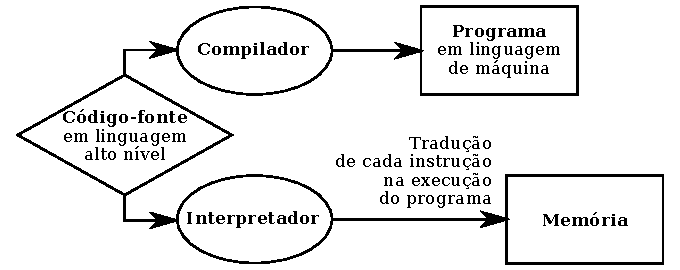
\includegraphics[width=.75\textwidth,keepaspectratio]{figures/compilador-interpretador.pdf}
  \caption*{\footnotesize Fonte: Produção do autor, adaptado de \citeonline{medina2006etal}.}
\end{figure}

Passando por um processo de entendimento de elementos mínimos no código, ignorando outros e agrupando em símbolos especificados, a compilação se inicia. Além dessa análise também é necessária a verificação se esses grupos estão em ordem ou outros erros possíveis. \citeonline{delamaro2004} descreve que código fonte de entrada termina tendo como saída o programa objeto, o compilador converte a linguagem simples em uma linguagem entendida pela máquina. Na Figura \ref{fig:compilador} é possível visualizar um compilador, somente com a principal etapa e dela as análises: Léxica, Sintática e Semântica.

\begin{figure}[h]
  \caption{Análises de um compilador}\label{fig:compilador}
  \centering

\includegraphics[width=.98\textwidth,height=10cm,keepaspectratio]{figures/etapas-compilador.pdf}
  \caption*{\footnotesize Fonte: Produção do autor, adaptado de \citeonline{ferrandin2005etal}.}
\end{figure}

\subsection{Processo de compilação}

Num compilador ideal, de acordo com \citeonline{aho2007etal} e visto na Figura \ref{fig:fullcompiler}, pode-se identificar a etapa de \textbf{análise} (\textit{front end}) e a etapa de \textbf{síntese} (\textit{back end}). Na síntese a partir da árvore sintática são geradas representações intermediárias até o programa alvo executável através de: geração de código intermediário, otimização de código e por fim o gerador de código. Durante todo o processo a tabela de símbolos guarda informação sobre nomes declarados e o tratamento de erros que age na etapa de análise, por exemplo, identificando erro e em qual linha.

\begin{figure}[h]
  \caption{Compilador completo}\label{fig:fullcompiler}
  \centering
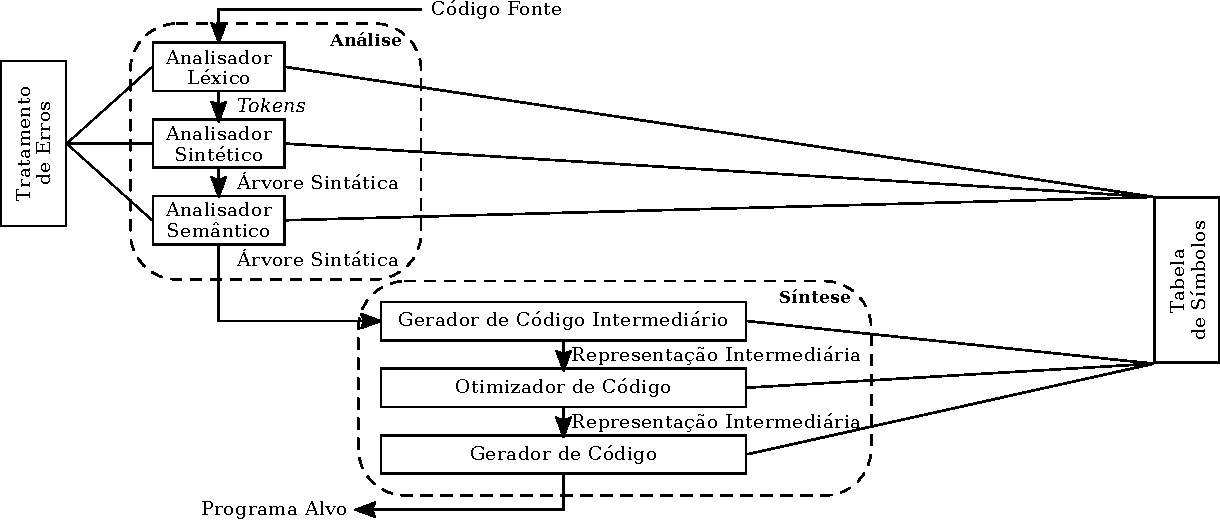
\includegraphics[width=\textwidth,keepaspectratio]{figures/compilador-completo.pdf}
  \caption*{\footnotesize Fonte: Produção do autor, adaptado de \citeonline{aho2007etal}.}
\end{figure}

%\subsection{Análise Morfológica}
%
\subsection{Análise Léxica}

A análise léxica (\textit{scanner}) é citada por \citeonline{aho2007etal} como sendo onde elementos mínimos (\textit{tokens}) são identificados, cada letra, número e outros caracteres (como pontuação e demais símbolos), além do espaço. Após reconhecidos, esses \textit{tokens} são então agrupados em lexemas: identificadores, palavras-chave reservadas, comandos, operadores, constantes, conjunto de texto, nome de variáveis, início e fim do algoritmo ou de blocos. Essa análise também ignora comentários e marcas de edição (tabulações, caracteres de avanço de linha e espaços). No Quadro \ref{qua:print} é dado uma linha do algoritmo para na Tabela \ref{tab:lexemas} apresenta os lexemas identificados.

\begin{quadro}[h]
\centering
  \caption{Exemplo para entendimento de tradutor}\label{qua:print}
\begin{lstlisting}[language=ual,frame=single]
  imprima "Aprendendo Algoritmo";
\end{lstlisting}
  \caption*{\footnotesize Fonte: Produção do autor, 2016.}
\end{quadro}

\begin{table}[h]
\centering
  \caption{Lexemas encontrados no exemplo}\label{tab:lexemas}
\begin{tabular}{ c | l }\hline
\textbf{Lexema} & \textbf{Classificação} \\ \hline
\texttt{imprima} & identificador da expressão de impressão \\ \hline
\texttt{"Aprendendo Algoritmo"} & conjunto literal de texto \\ \hline
\texttt{;} & caractere de encerramento de expressão \\ \hline
\end{tabular}
  \caption*{\footnotesize Fonte: Produção do autor, 2016.}
\end{table}

\subsection{Análise Sintática}

Análise sintática (\textit{parser}), recebe a sequência de lexemas da análise anterior e determina se são elementos estruturais pertencentes à linguagem desejada, exposto por \citeonline{delamaro2004}. Esses elementos são estruturados de modo ramificado (Figura \ref{fig:ast}), dando origem ao termo árvore sintática. São essas estruturas: expressões aritméticas, comandos de atribuição ou declarações de procedimentos e as relações entre eles, garantindo que seja correto sintaticamente.

\begin{figure}[h]
  \caption{Exemplo de árvore sintática}\label{fig:ast}
  \centering
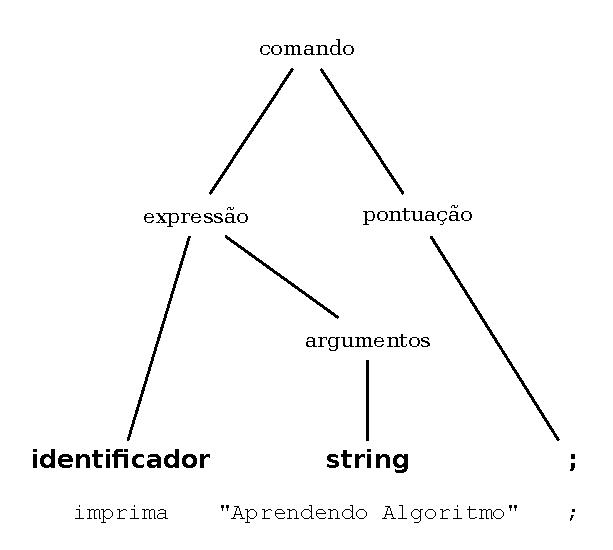
\includegraphics[width=.65\textwidth,height=10cm,keepaspectratio]{figures/ast.pdf}
  \caption*{\footnotesize Fonte: Produção do autor, 2016.}
\end{figure}

\subsection{Análise Semântica}

A análise semântica verifica o ``significado'' das instruções, ao tratar de aspectos relacionados à sua ordem. Esta análise confere se há sentido de acordo com a gramática definida pela linguagem, para a correta execução. É possível que um programa esteja em acordo com a sintaxe gramatical, porém erros quanto a semântica são apresentados. A gramática da linguagem é utilizada nesta etapa, ela pode ser representada em uma árvore gramatical (\textit{tree grammar}). Por exemplo se só for possível imprimir conjuntos literais de texto, variáveis, conjuntos dessas ou operações aritméticas entre parênteses e for criado como impressão direta de um número.

\section{Ferramentas para algoritmos}
% Ferramentas para prática de algoritmos

Ferramentas computacionais para prática de algoritmos são utilizadas no processo de ensino aprendizagem com enfoques variados. Várias dessas ferramentas podem ser listadas:

\begin{itemize}

\item \textbf{ILA + AMBAP}: Desenvolvida por \citeonline{evaristo2000} o Interpretador de Linguagem Algorítmica (ILA) é do um tradutor do tipo CLI e foi utilizado para simulação dos algoritmos no editor gráfico AMBAP (AMBiente para Aprendizado e Programação);

\item \textbf{UAL + EditorUAL}: Desenvolvido por \citeonline{spallanzani2000etal} na UNESA é basicamente um tradutor do tipo CLI, desenvolvido para linux. Ele foi posteriormente portado para Windows, e neste sistema operacional foi criado o EditorUAL do tipo GUI;

\item \textbf{VisuAlg}: Desenvolvida por Claudio Morgado de Souza, programador e analista, bem como professor universitário, é um ferramenta utilizada tanto em cursos técnicos quanto em meio universitário. A facilidade de obtenção do seu executável para Windows e documentação completa são atrativos, além de sua  simplicidade sem perder funções úteis para iniciantes \cite{souza2013etal};

\item \textbf{Web Portugol}: Desenvolvida por pesquisadores na UNIVALI permite o acesso via navegadores que tenham integração com Java, desde que o mesmo também esteja instalado no computador \cite{souza2013etal};

\item \textbf{Construtor}: Desenvolvido pelo Centro Educacional de Informática Aplicada do SENAC (Rio de Janeiro), é a primeira ferramenta para algoritmos com interface gráfica encontrada para uso em Windows. Esta ferramenta tem a vantagem de acompanhar o livro ``Construção de Algoritmos'' de \citeonline{fernandes1999etal}.

\end{itemize}

Na Tabela \ref{qua:compare-tools} consta um comparativo de pontos que ressaltam como fatores determinantes em escolha de qual opção utilizar pelo educador no ensino, para que seus alunos pratiquem o conteúdo.

\begin{table}[h]
\centering
\caption{Comparativo das ferramentas}\label{qua:compare-tools}
\resizebox{\textwidth}{!}{%
\begin{tabular}{ r | l | l | l | l | l }\hline
& UAL+Editor & ILA+AMBAP & VisuAlg & Web Portugol & Contrutor \\ \hline
Plataforma & Linux e Windows & DOS/Windows & Windows & Web (Java Applet) & Windows \\ \hline
Licença & \textit{open source} & \textit{freeware} & \textit{freeware} & \textit{open source} & \textit{open source} \\ \hline
Instituição & UNESA & UFAL &  & UNIVALLI & SENAC \\ \hline
Linguagem & Haskell & Java (editor) &  & Java & \\ \hline
\end{tabular}%
}
  \caption*{\ifdraft{\color{green}}{}\footnotesize Fonte: Produção do autor.}
\end{table}

Desenvolvida por \citeonline{esmin1998} quando vinculado a UNOESC o \textbf{Portugol/Plus} é a mais antiga opção encontrada no Brasil. Merecendo destaque por ser comumente referenciada por outros autores, inclusive quando tratam sobre desenvolvimento de novas soluções. Porém por ser em plataforma \textit{Disk Operating System (DOS)}, inclusive com interface gráfica foi desconsiderada no levantamento acima.

Ao delimitar a quantidade de itens outras também não foram listadas, alguns casos o acesso ao programa para testes não estava disponível ou menor relevância na literatura. No entanto  merecem menção: \textbf{PascalX}, por Athur Vargas Lopes da ULBRA; \textbf{Web-UNERJOL}\nocite{ferrandin2005etal}, utilizando UNERJOL os dois pelo mesmo acadêmico na UNERJ com colaborações distintas.
%PascalX\nocite{http://www.ulbra.tche.br/~avl/home.htm}

Outras mais não foram consideradas por fugirem do escopo ao utilizar robótica, jogos, foco em estrutura de dados ou similares: Guido VanRobot, Robot Prog, Kids Ruby, Fut Code, TBC-AED. Eram pretendidas somente ferramentas com pseudo-linguagem algorítmica em português, preferencialmente Portugol, partindo novamente do Editor UAL como referencial.
%TBC-AED: por pesquisadores da Universidade Federal de Lavras/Departamento de Ciências da Computação em Minas Gerais

\section{Caso de Ensino com Livro e Ferramenta}

O livro ``Introdução à programação: 500 algoritmos resolvidos'' de \citeonline{lopes2002etal} tem um grande apelo por seu elevado número resoluções como seu título deixa claro. Isso motiva os educadores utilizarem como livro texto base de disciplinas de ensino de Lógica da Programação. Neste livro todos os algoritmos propostos para execução computadorizada estão impressos na sintexe UAL - variante do Portugol - acompanha mídia ótica que contém os exercícios nesta e também em ILA. Na Tabela \ref{tab:compare-ualila} é visto a comparação entre elas.

%\the\textwidth
%455.0pt
%\halftextwidth
%227.7pt
%\noindent
\begin{table}[h]
\centering
  \caption{Comparação entre UAL e ILA}\label{tab:compare-ualila}
\begin{tabular}{p{75mm} | p{75mm}}\hline
\multicolumn{1}{c|}{\textbf{Em UAL}} & \multicolumn{1}{c}{\textbf{Em ILA}} \\ \hline
\begin{lstlisting}[language=ual,style=table]
prog algoritmo11
  imprima "Aprendendo Algoritmo!!!";
fimprog
\end{lstlisting} &
\begin{lstlisting}[language=ila,style=table]
//prog algoritmo11
inicio
  limpar
  escrever "Aprendendo Algoritmo!!!"
fim
\end{lstlisting} \\ \hline
\end{tabular}
  \caption*{\ifdraft{\color{green}}{}\footnotesize Fonte: Produção do autor, a partir dos exemplos de \citeonline{lopes2002etal}.}
\end{table}

Todo o projeto está pautado neste algoritmo simplista, obtido em \citeonline[p.~26]{lopes2002etal} e na mídia que acompanha o livro destes autores. Facilmente se nota a diferença nos blocos de início e fim do programa, além de somente em UAL ter o nome do mesmo (solucionado com uso de linha comentada) e o comando de limpeza somente necessário em ILA. As chamadas de escrita em tela também têm sua palavra reservada diferente. Nenhuma delas delimita o argumento por parênteses e UAL exige ponto e vírgula ao final. As duas não são sensíveis no uso de letras maiúsculas ou minúsculas nas palavras chaves .

\begin{table}[h]
\centering
  \caption{Escopo das linguagens UAL e ILA}\label{tab:escopo-lang}
\begin{tabular}{lC{40pt}|C{40pt}}
\cline{2-3}
 & \textbf{UAL} & \textbf{ILA} \\ \hline
\multicolumn{1}{l|}{Saída em tela} & \textbf{s}im & \textbf{s}im \\ \hline
\multicolumn{1}{l|}{Entrada de argumentos} & \textbf{s}im & \textbf{s}im \\ \hline
\multicolumn{1}{l|}{Tipos de dados} & \textbf{s}im & \textbf{s}im \\ \hline
\multicolumn{1}{l|}{Variáveis} & \textbf{s}im & \textbf{s}im \\ \hline
\multicolumn{1}{l|}{Atribuições} & \textbf{s}im & \textbf{s}im \\ \hline
\multicolumn{1}{l|}{Operações aritiméticas} & \textbf{s}im & \textbf{s}im \\ \hline
\multicolumn{1}{l|}{Operações relacionais} & \textbf{s}im & \textbf{s}im \\ \hline
\multicolumn{1}{l|}{Estruturas de controle} & \textbf{s}im & \textbf{s}im \\ \hline
\multicolumn{1}{l|}{Vetores} & \textbf{s}im & \textbf{s}im \\ \hline
\multicolumn{1}{l|}{Matrizes} & \textbf{n}ão & \textbf{s}im \\ \hline
\multicolumn{1}{l|}{Funções} & \textbf{n}ão & \textbf{s}im \\ \hline
\end{tabular}
  \caption*{\ifdraft{\color{green}}{}\footnotesize Fonte: Produção do autor, baseado em \citeonline{spallanzani2000etal,evaristo2000}.}
\end{table}

Sendo as estruturas de um algoritmo o escopo da linguagem, há diferenças entre UAL e ILA também quando quanto sua abrangência, visto Tabela \ref{tab:escopo-lang} sendo a primera estrutura única que o presente trabalho abrange. Não tendo a UAL estruturas como matrizes n-dimensionais, funções com ou sem passagem de parâmetros, novos comandos para tomada de decisões e controle de repetições, novos tipos de dados, conversores de tipos \cite{spallanzani2000etal}.

\ifdraft{}{
%\subsection{Ensino Aprendizagem}

% NOTE citar Teoria das Inteligências Múltiplas de Gardner

%\section{Pseudoliguagem e Portugol}


%
%
%
%
%
%\item G-Portugol
%
%\item Portugol IDE
%
%\item Portugol Studio
%
%\item ASA
%
%\item ATMUF
%
%\item AWTM
%
%\item AMBAP
%
%\item CIFluxProg
%
%\item RAFF
%
%\item SistLog
%
%\item Ambiente SICAS
%
%\item C-Tutur
%
%\item PL-Detective

%\end{itemize}

%\subsection{UAL e Editor UAL}

%\subsection{Demais Aplicativos}
%
%%\subsection{Plataforma Digitais de Ensino}
%\subsection{Ambiente Virtual de Aprendizagem - AVA}
%
%% NOTE Interactive Learning - Aprendizado Interativo {tonin2012etal}
%
%\subsubsection{Udacity}
%
%\subsubsection{Codeacademy}
%
%\subsubsection{SoloLearn}
%
%\subsubsection{Code School}
%
%\subsubsection{Kan Academy}
%
%\subsection{Programação em Blocos}
%
%\subsubsection{\textit{Blockly}}
%
%\section{\textit{Online Judge}}
%
%Sistema de Apoio a Competições de Programação é a denominação em português de
%\textit{Online Judge} por \citeonline{campos2004etal}, nomeado como BOCA.
%E mais recente foi desenvolvido por acadêmico da URI (Universidade Regional
%Integrada do Alto Uruguai e das Missões) com base nesse trabalho anterior o URI
%\textit{Judge Online} \cite{tonin2012etal}.
%
%\section{Tecnologias Web}
%
%\subsection{Linguagem de Marcação de Texto}
%
%\subsection{Liguagem de Programação para Web}
%
%\subsubsection{ECMAScript}
%
%\subsubsection{WebAssembly}
%
%\subsection{Navegadores Web}
%
%\subsection{Aprimoramentos para Uso \textit{Offline}}
}
